\documentclass[10pt,letterpaper]{article}
\usepackage[margin=1in]{geometry}
\usepackage{fancyhdr}
\usepackage[utf8]{inputenc}
\usepackage{palatino}
\usepackage{microtype}
\usepackage{hyperref}
\usepackage{graphicx}
\usepackage[hang,bf,small]{caption}
\usepackage{amsmath,amssymb,amsthm}

\setlength{\parindent}{0cm}
\setlength{\parskip}{1em}

\hypersetup{colorlinks,
	linkcolor = black,
	citecolor = black,
	urlcolor  = black}
\urlstyle{same}

\begin{document}

\begin{titlepage}
	\vspace*{4cm}
	\begin{flushright}
	{\huge
		Cattlestar Balactica \\ [1cm]
	}
	{\large
		ENGR 421 -- Design Concept Proposal \\ [3cm]
	}
	\end{flushright}

	\begin{flushright}
	Soo-Hyun Yoo
	\end{flushright}

\end{titlepage}

\newpage

\section*{Design Concepts}

\subsection*{Simply Awesome}

Our team name, Cattlestar Balactica, originates from one of my deranged,
sleep-deprived rants about space and robots. As such, our robot will be
reminiscent of a Cylon Raider (Figure~\ref{fig:raider}), complete with an
oscillating red eye that will aid the computer vision system.

\begin{figure}[!h]
	\centering
	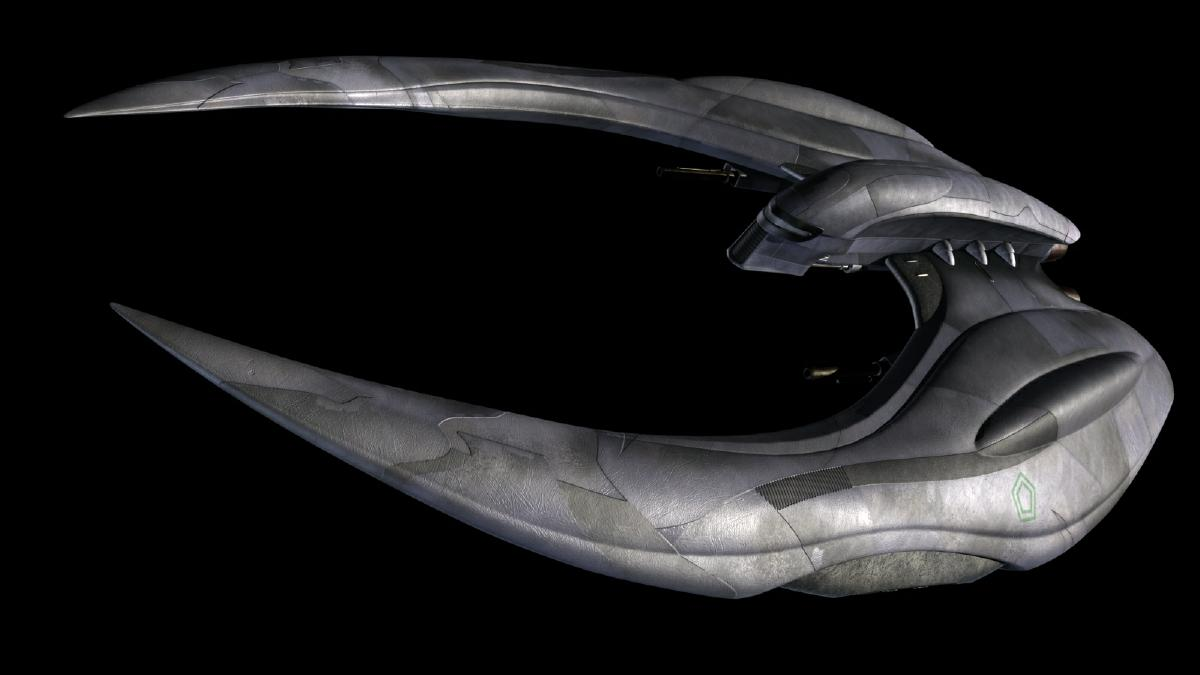
\includegraphics[width=0.8\textwidth]{raider.jpg}
	\caption{A Cylon Raider}
	\label{fig:raider}
\end{figure}

\subsection*{Mechanical Shooter}

There are three viable ways of shooting a BB:

\begin{itemize}
	\item Magnetically (coilgun style): This is cool, but keeping a bank of
		capacitors charged at the correct voltage level, correctly building
		a series of coils, firing the coils (and turning them off) at precisely
		the right times, and accounting for the heat buildup in the coils is
		going to be too much work.
	\item Pneumatically: Compressed air is a powerful, consistent source of
		energy, but we don't have easy, portable access to pressurized air. We
		could use paintball CO$_2$ canisters, but making sealed fittings for
		them that are easy to put together and safe to maintain may take some
		work.
	\item Mechanically: There are two options:
		\begin{itemize}
			\item Cock-and-reload with spring: This is slow and loud.
			\item Spinning wheel: This is quiet, compact, consistent, and
				allows for (literally) the maximum rate of fire. If the wheel
				is equipped with a rotary encoder, any transfer of energy to
				a BB entering the chamber can easily be countered, maintaining
				rotational velocity (Figure~\ref{fig:shooter}).
		\end{itemize}
\end{itemize}

\begin{figure}[!h]
	\centering
	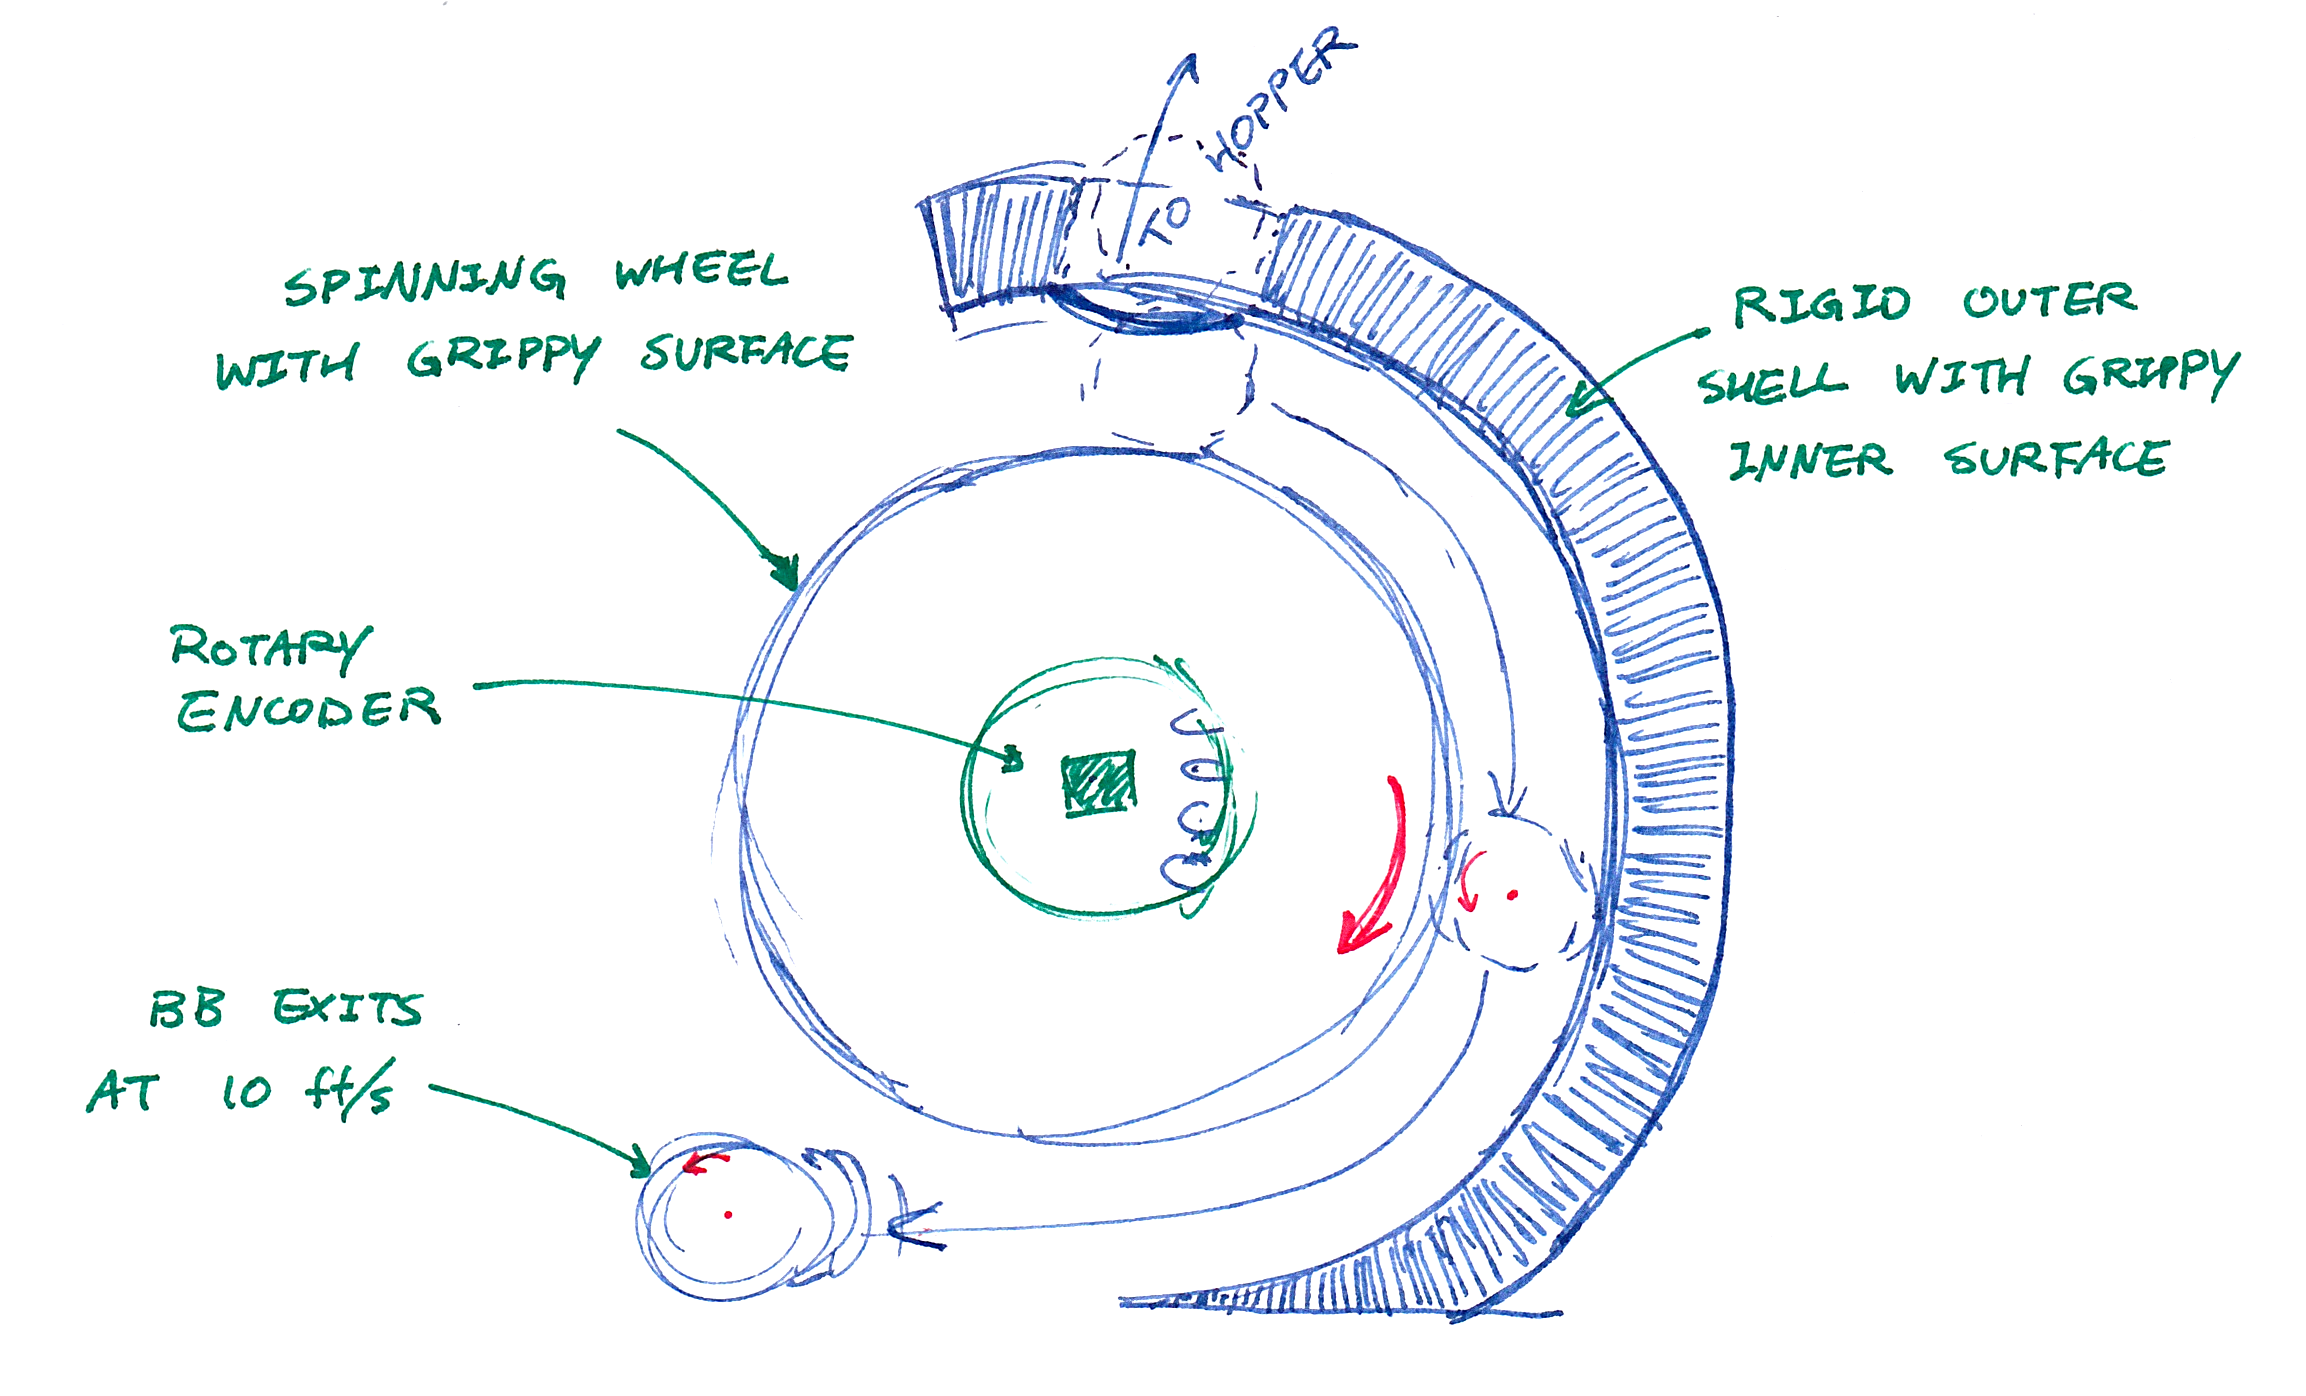
\includegraphics[width=0.8\textwidth]{shooter_side.png}
	\caption{Side view of shooter. The inner wheel is powered by a motor whose
	position is tracked by a magnetic rotary encoder.}
	\label{fig:shooter}
\end{figure}

The spinning wheel method of shooting BBs is much preferred over the others for
the reasons specified above.

\subsection*{Impeccable Aim}

There are three viable ways to aim the shooter:

\begin{itemize}
	\item Linear slide: This provides full coverage of the board. There are
		three mechanisms that achieve linear motion:
		\begin{itemize}
			\item Pneumatics: Fast and sounds cool, but the magnet inside the
				cylinder slips with little force, so high acceleration will be
				impossible.
			\item Ball screw: May be fast with a fast enough motor.
			\item Timing belt and pulley: Fast, quiet, lighter than ball screw.
		\end{itemize}

	\item Pivoting (the shooter): This will result in a small, simple robot in
		one of few ways:
		\begin{itemize}
			\item Servo: Backlash will be a problem, and common off-the-shelf
				servos are either strong and slow or weak and fast. The fastest
				servos are still only 0.05 s/60 degrees. Especially considering
				the inertia of the shooter, a servo may not be strong enough.
			\item Something else: No.
		\end{itemize}

	\item Deflecting the BBs (after they exit the shooter): Less mass can be
		moved more quickly than more mass. There are a few ways to deflect the
		BBs once they exit the shooter:
		\begin{itemize}
			\item Tube and servo: May flex too much, resulting in inconsistent aim.
			\item Fairly stiff but bendable rail and servo: Limited range
				(maybe 45 degrees), fragile.
			\item Electromagnet: Strong, rapid, consistent. Think CRT and
				electrons (except here, the electrons are BBs) (Figure~\ref{fig:em}).
		\end{itemize}
\end{itemize}

\begin{figure}[!h]
	\centering
	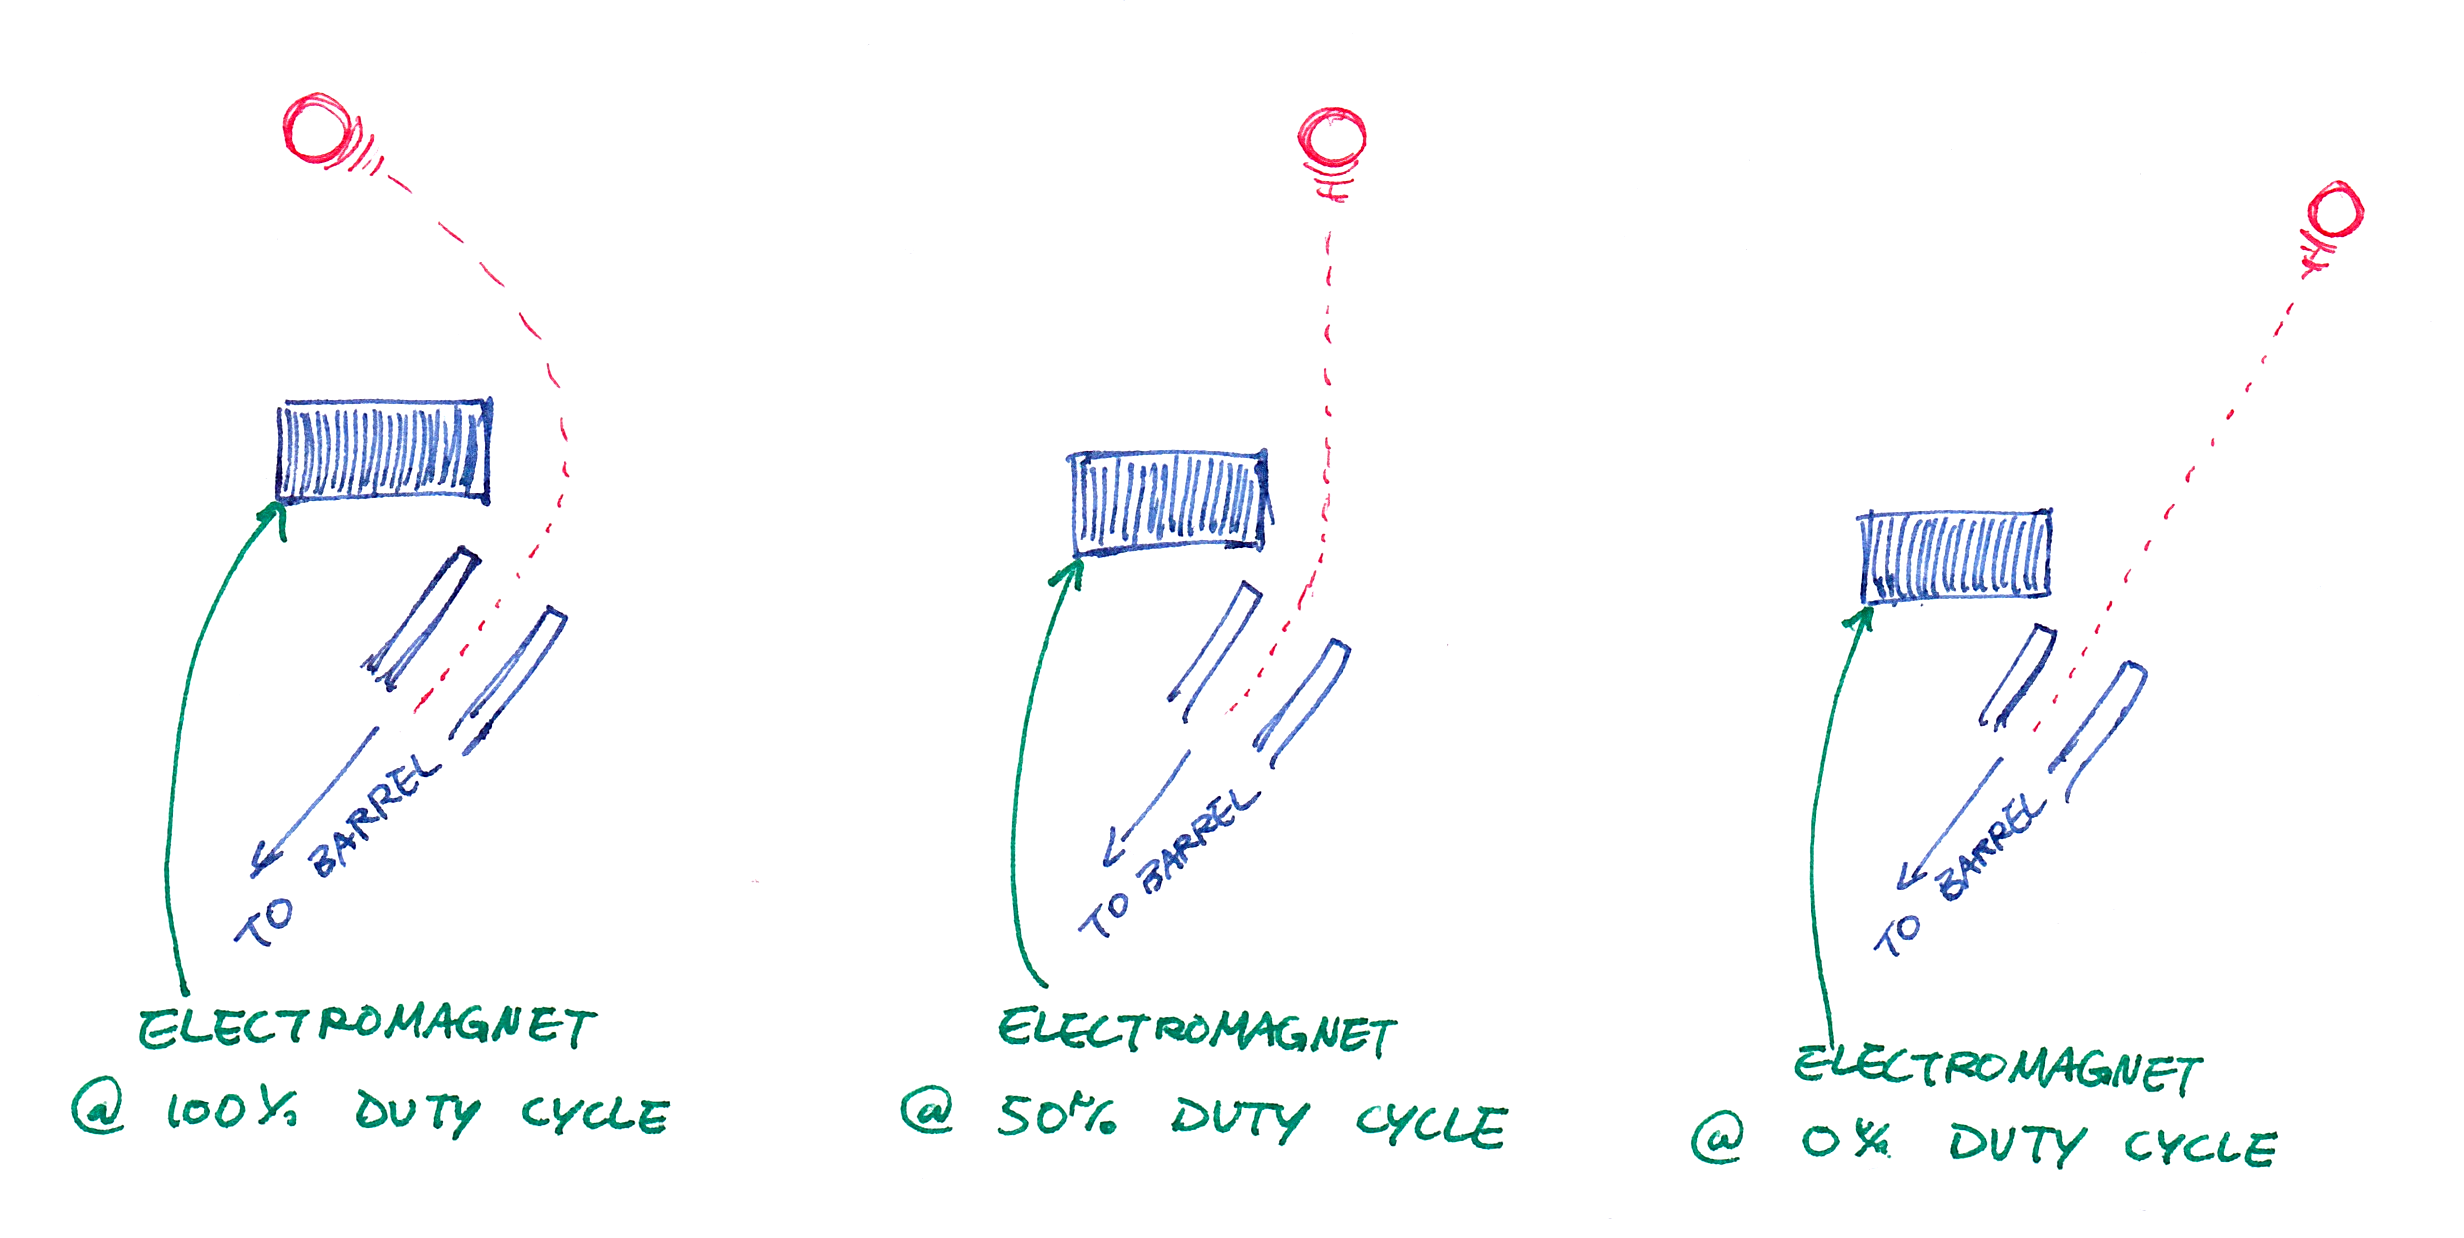
\includegraphics[width=0.7\textwidth]{electromagnet_top.png}
	\caption{Top view of electromagnet setup.}
	\label{fig:em}
\end{figure}

A magnet has already been ordered. Depending on its strength, we may either
have a magnet on either side of the shooter or have one on one side (as shown
in Figure~\ref{fig:em}).

\subsection*{Agitated Hopper}

In order to prevent BBs from jamming, the hopper will be agitated (much like
the way a washing machine agitates clothes). The hopper will be capable of
feeding BBs into the shooter at a known rate in order to avoid wasting BBs.

Additionally, a photogate will be used to determine whether or not the hopper
is empty. If we decide to employ multiple shooters, this will prevent the
system from trying to use a shooter that has run out of BBs.

Fortunately, the shooter design is such that once the BB is in the chamber,
there is no way for it to become jammed within the chamber.


\subsection*{Computer Vision}

OpenCV will be used for blob and edge detection and various filters. Because
the camera will be installed at an angle to the playing field, the image will
be rectified prior to any other calculations.

We will use the fastest off-the-shelf USB webcam to minimize motion blur.


\subsection*{Two Shooters}

Use of the electromagnet, combined with a high rate of fire, should be
sufficient for a single shooter to hit both pucks nearly simultaneously.
Nevertheless, redundancy is never a bad thing (and will multiply our potential
maximum rate of fire), so we will have at least two shooters.

A linear slide will allow us to move each shooter independently of each other
to either extremes of our end of the board.


\section*{Functional Goals}

Given that the maximum linear speed of the BBs is capped at an easily
attainable 10 ft/s, we must maximize performance in four other key areas, in
increasing order of importance:

\begin{itemize}
	\item Rate of fire. If we dump BBs fast and score both pucks before the
		other robot can empty their hopper, we effectively decrease the number
		of BBs the other team ``gets'' to use.
	\item Speed of redirection (of aim). Time spent changing the direction of
		fire and an inability to track a fast-moving puck will result in wasted
		time and BBs. Even if we are able to dump BBs faster than any other
		robot, if we fail to keep up with the puck, we may as well not shoot at
		all.
	\item Accuracy of aim. BBs must hit the puck when and where we want them
		to. The sensory system must accurately determine the location of the
		puck in order for the shooter to be effective.
	\item Real-time awareness of the game state. Even a perfect shooter will
		lose us the game if every action comes a half-second later than the
		reality upon which it was based. Minimizing the time between image
		capture and action will be of utmost importance.
\end{itemize}


\newpage
\section*{Sketch of System}

\begin{figure}[!h]
	\centering
	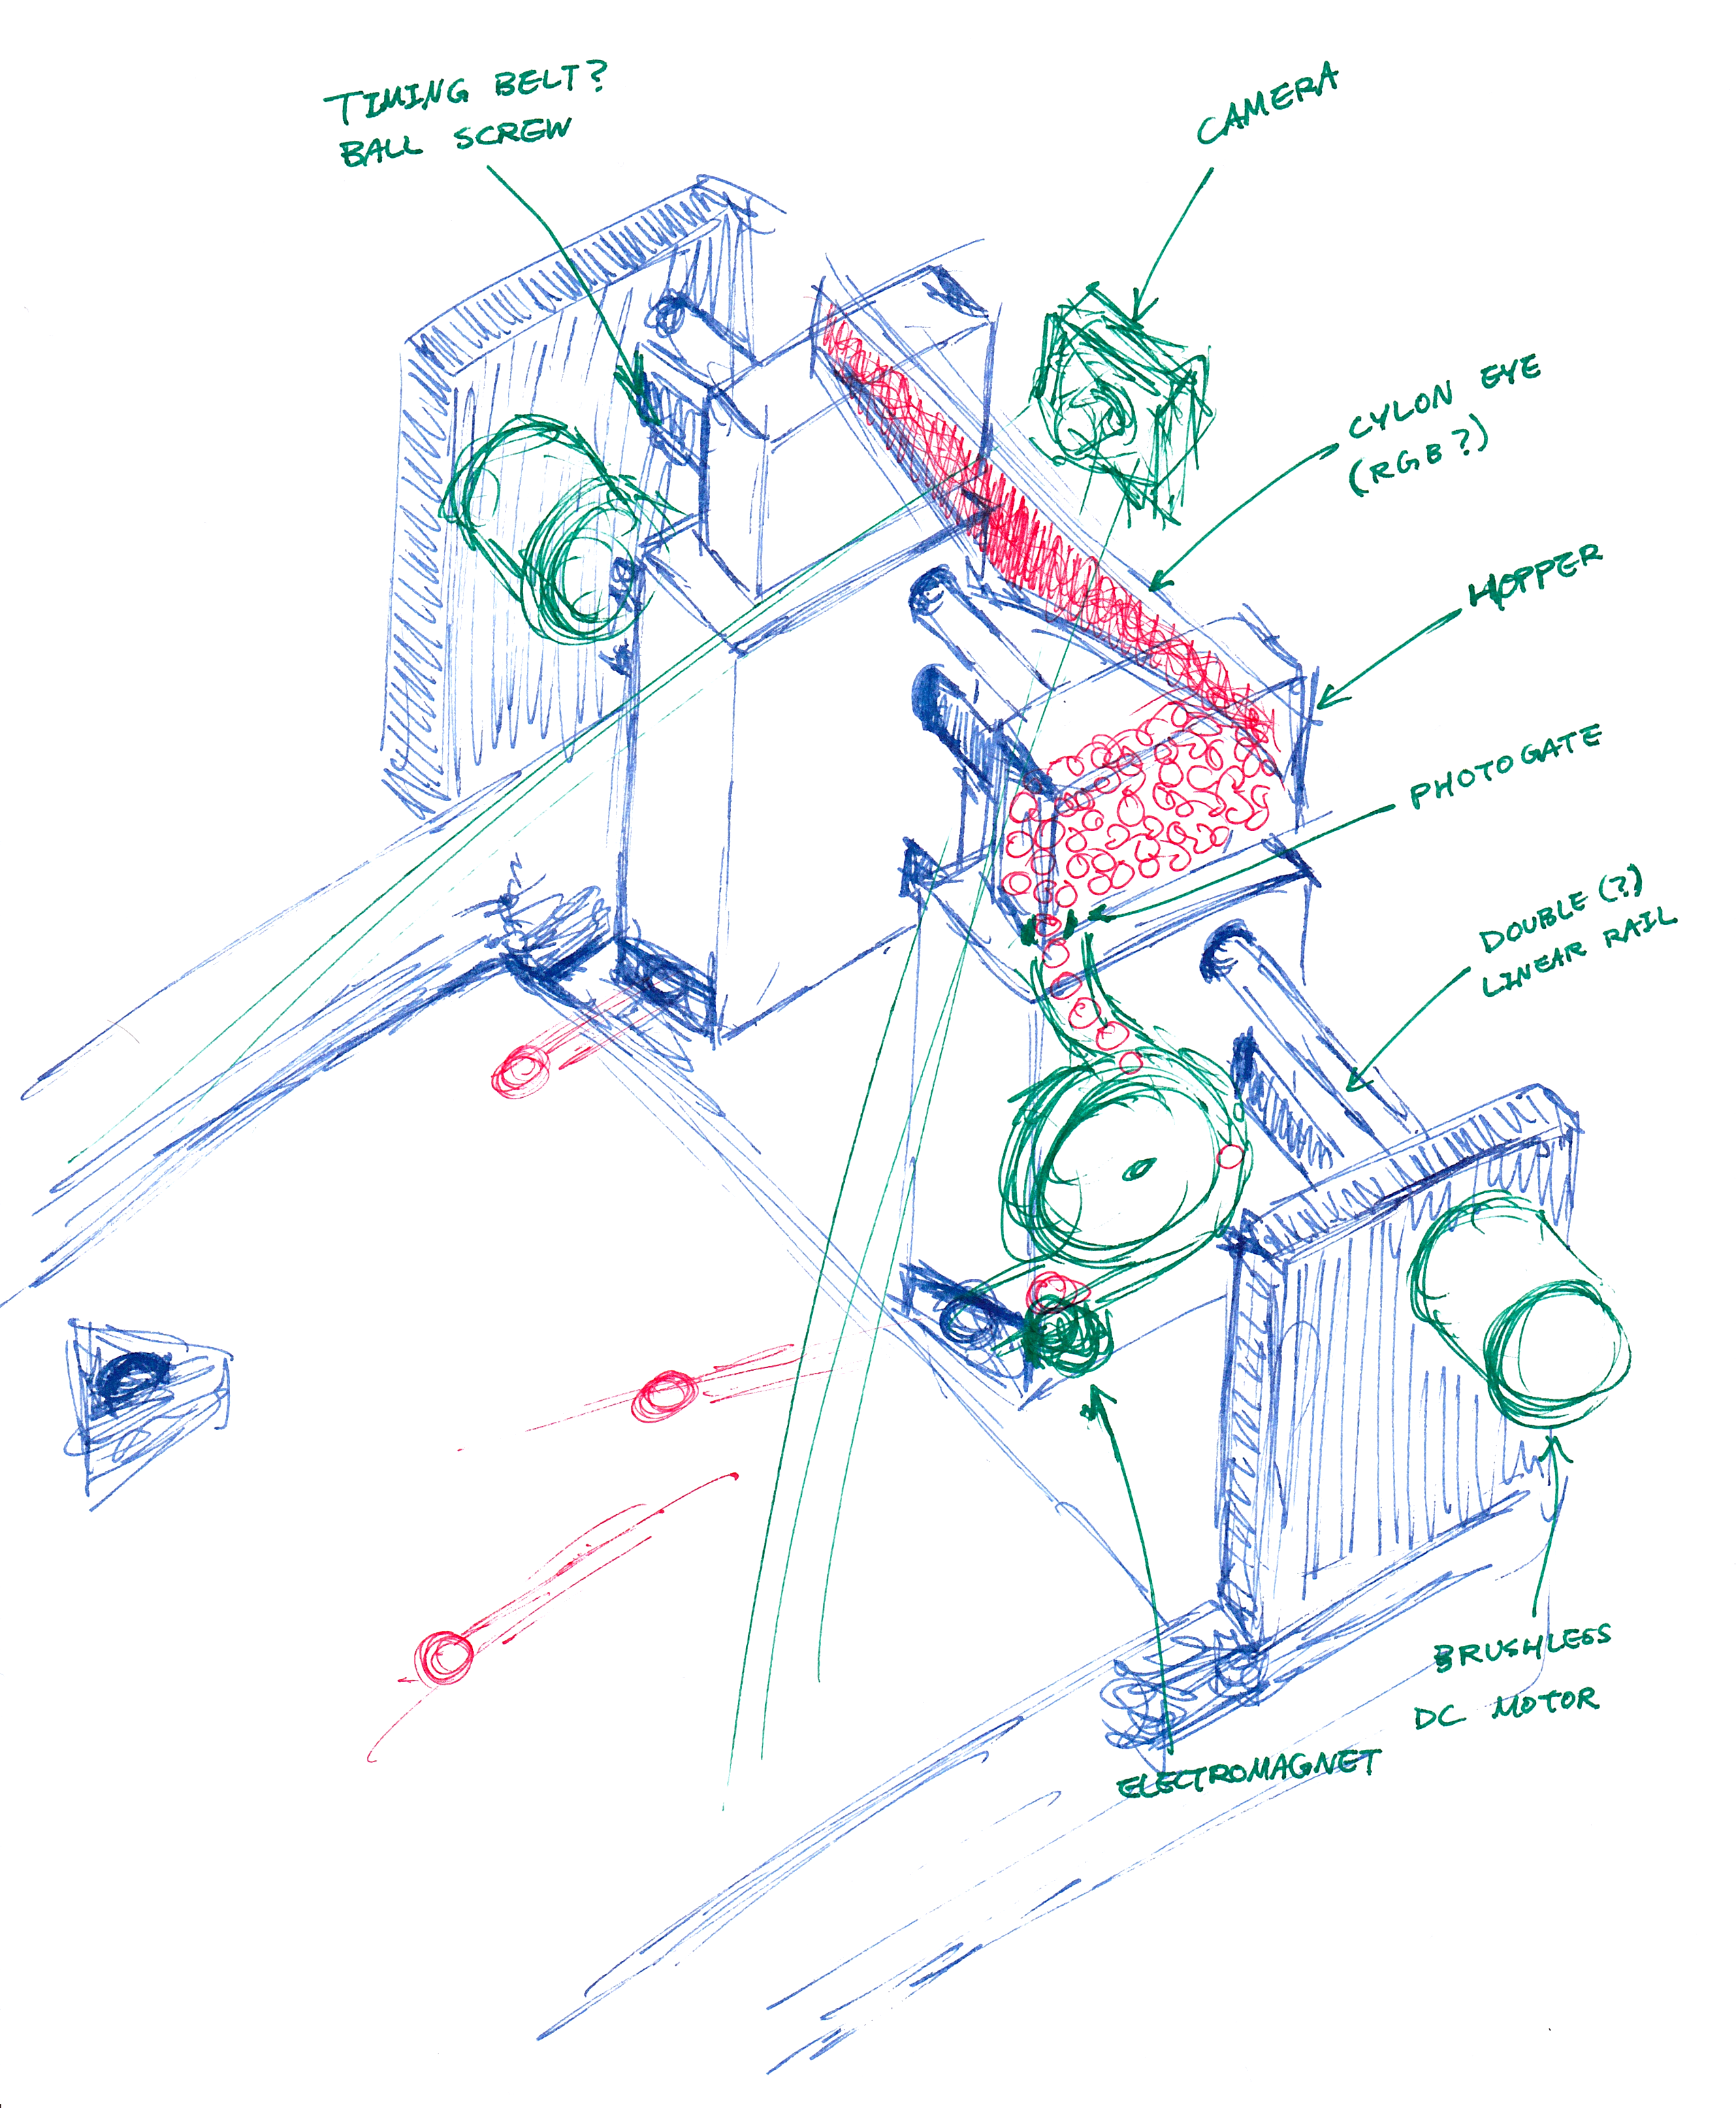
\includegraphics[width=0.9\textwidth]{robot_overview.png}
	\caption{Overview of robot.}
	\label{fig:robot}
\end{figure}


\newpage
\section*{Functional Flowchart}

\begin{figure}[!h]
	\centering
	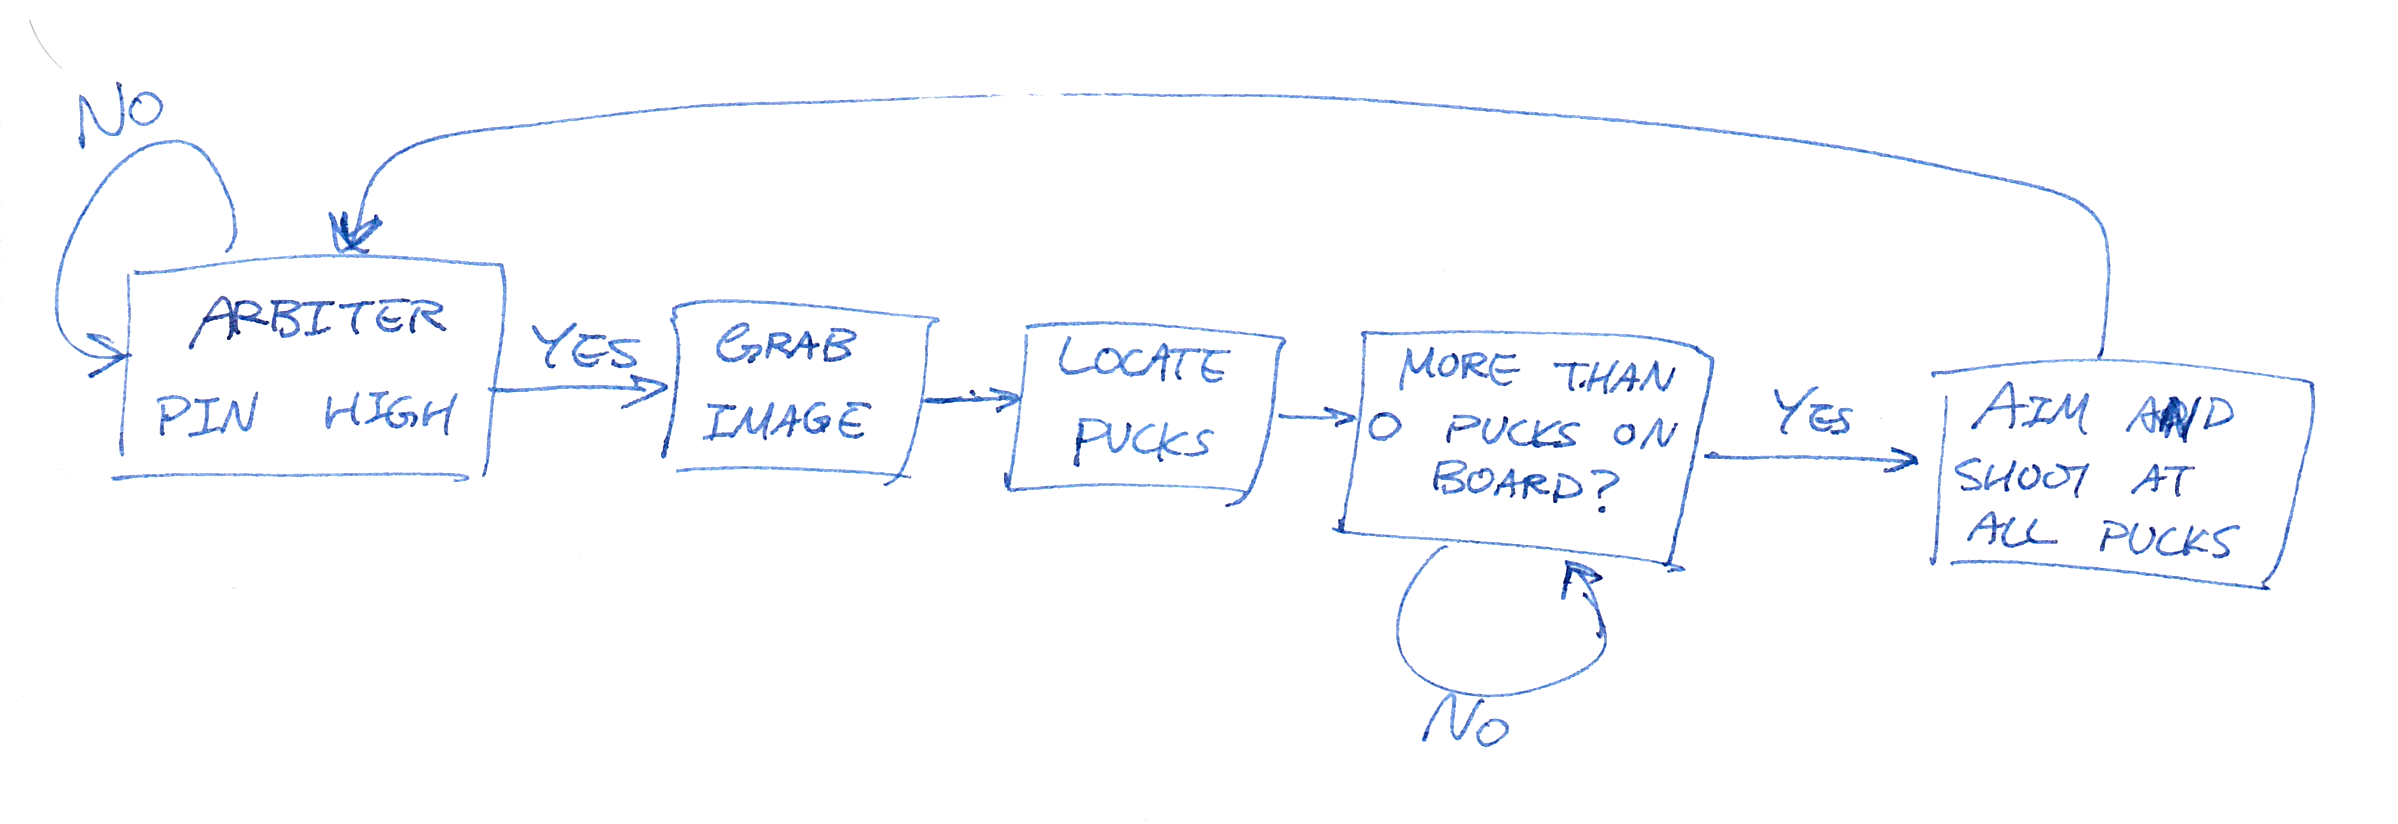
\includegraphics[width=1.0\textwidth]{flowchart.png}
	\caption{Functional flowchart.}
	\label{fig:flowchart}
\end{figure}


\section*{Block Diagram}

\begin{figure}[!h]
	\centering
	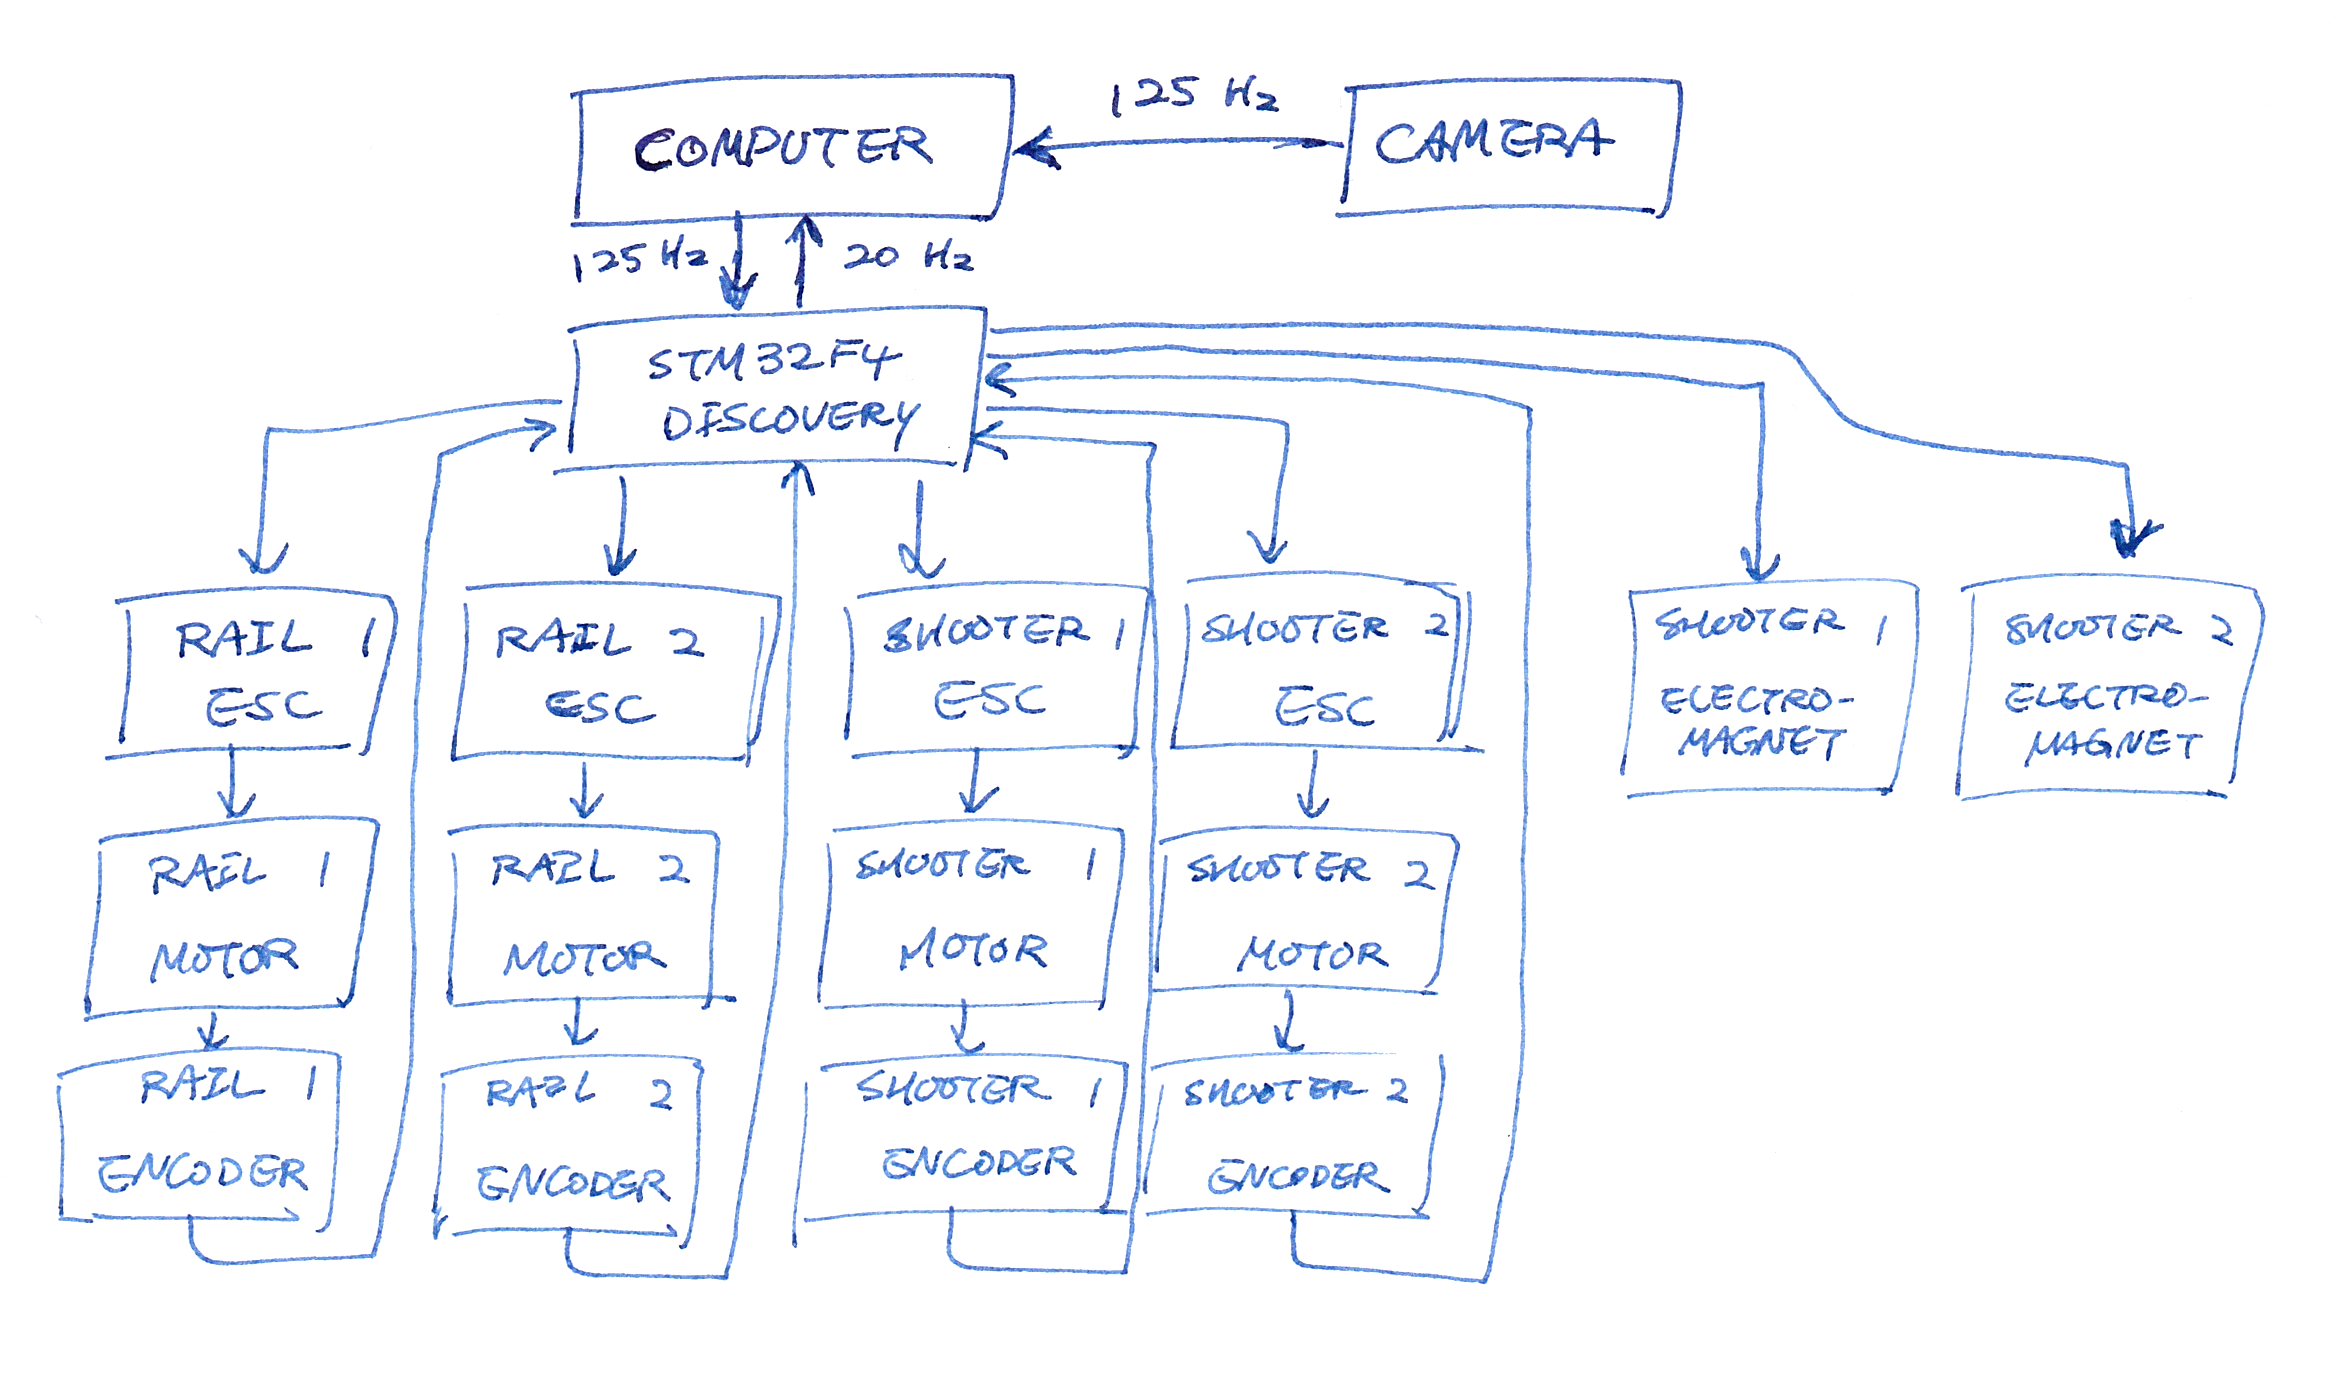
\includegraphics[width=1.0\textwidth]{block_diagram.png}
	\caption{Block diagram.}
	\label{fig:block}
\end{figure}


\newpage
\section*{Primary Responsibilities}

As the computer scientist on the team, I will be responsible for all code,
including the vision system as well as any embedded code necessary for
controlling motors and reading sensors.

I will also be designing and implementing most of the electrical system.


\section*{Initial Plan of Action}

A prototype shooter and hopper has already been constructed. A revised version
will be manufactured over the upcoming week.

An electromagnet and encoder breakout boards have been shipped from their
respective vendors. These will arrive on Saturday and be tested next week.


\end{document}

